%%%%%%%%%%%%%%%%%%%%%%%%%%%%%%%%%%%%%%%%%%%%%%%%%%%%%%%%%%%%%%%%%%%%%%%%%%%%%%
% courseplan.tex — Course Plan for 247-519-VA
% Compiles standalone: pdflatex courseplan.tex (×2)
% Uses the Sparkle class located one directory above.
%%%%%%%%%%%%%%%%%%%%%%%%%%%%%%%%%%%%%%%%%%%%%%%%%%%%%%%%%%%%%%%%%%%%%%%%%%%%%%
\documentclass[twoside]{../Sparkle}

% ─── Metadata ────────────────────────────────────────────────────────────────
\documenttitle{Course Plan: Project Planning \& Prototyping}
\authorname{J. F. N. Salik,}
\authoremail{salikj@vaniercollege.qc.ca}
\authortitle{Instructor, Computer Engineering Technology}
\documentID{247-519-VA}
\copyrightyear{2026}
\authoraddress{%
    \color{vanierred}\textbf{Department of Computer\\
    Engineering Technology}\normalcolor\\%
    Vanier College\\%
    821 Sainte-Croix Avenue\\%
    Saint-Laurent, Qu\'{e}bec\quad H4L~3X9}

\definecolor{vanierred}{RGB}{195,0,47}

% ─── Packages ────────────────────────────────────────────────────────────────
\usepackage{amsmath,amssymb}
\usepackage{booktabs}
\usepackage{graphicx}
\usepackage{longtable}
\usepackage{array}
\usepackage{ragged2e}
\usepackage[hidelinks]{hyperref}

\setcounter{tocdepth}{2}

% ─── Column types for the weekly schedule table ───────────────────────────
\newcolumntype{L}[1]{>{\RaggedRight\arraybackslash}p{#1}}

%%%%%%%%%%%%%%%%%%%%%%%%%%%%%%%%%%%%%%%%%%%%%%%%%%%%%%%%%%%%%%%%%%%%%%%%%%%%%%
\begin{document}

% ─────────────────────────────────────────────────────────────────────────────
\chapter*{Course Plan}
\addcontentsline{toc}{chapter}{Course Plan}
% ─────────────────────────────────────────────────────────────────────────────

\section*{Course Identification}
\addcontentsline{toc}{section}{Course Identification}

\begin{tabular}{@{}ll@{}}
\textbf{Course title}     & Project Planning \& Prototyping \\
\textbf{Course number}    & 247-519-VA \\
\textbf{Credits}          & 3 (3-2-3: 3 hours lecture, 2 hours lab, 3 hours homework) \\
\textbf{Prerequisite}     & 247-418-VA (Embedded Systems II) or instructor consent \\
\textbf{Term}             & Fifth semester, Computer Engineering Technology \\
\textbf{Instructor}       & J. F. N. Salik \\
\textbf{Contact}          & \texttt{salikj@vaniercollege.qc.ca} \\
\end{tabular}

\bigskip

\section*{Course Description}
\addcontentsline{toc}{section}{Course Description}

Students develop and validate a functioning IoT prototype subsystem over one semester,
applying industry product-development methods at each stage.
The course positions itself within the \emph{Stage-Gate} model used by engineering firms:
students enter at Gate~2 (concept selected) and exit at Gate~3 (prototype validated and
documented). Every chapter delivers one \emph{Portfolio Entry} --- a short, structured
document section --- that accumulates into a complete prototype-documentation package
submitted at Milestone~3.

Three graded milestones track progress:
\begin{enumerate}
\item \textbf{Milestone~1 --- Specification Review (end of Week~6):}
      Portfolio Entries 1--9 assembled. Design decisions locked.
\item \textbf{Milestone~2 --- Build Review (end of Week~9):}
      Prototype built and validated against specifications. Planning artefacts complete.
\item \textbf{Milestone~3 --- Gate~3 Presentation (end of Week~12):}
      Final live presentation (10--15 min) plus complete documentation package
      submitted. This is the Gate~3 exit submission.
\end{enumerate}

\bigskip
\noindent\textbf{Running example.}\quad
All lecture examples use a single IoT robotic sorting subsystem throughout the course
(selling price $p = \$1{,}200$~CAD, variable cost $c_\mathrm{var} = \$480$~CAD,
BOM~$= \$124.85$~CAD, $C_\mathrm{fixed} = \$8{,}000$~CAD).
Students apply the same methods to their own chosen project.

\section*{Stage-Gate Context}
\addcontentsline{toc}{section}{Stage-Gate Context}

Figure~\ref{fig:cp-stagegate} places the course within the five-stage product-development
model.  Students enter with a defined concept (Gate~2) and spend the semester building the
evidence needed to pass Gate~3: a validated prototype, a costed BOM, and a documented
design history file.

\begin{figure}[h]
\centering
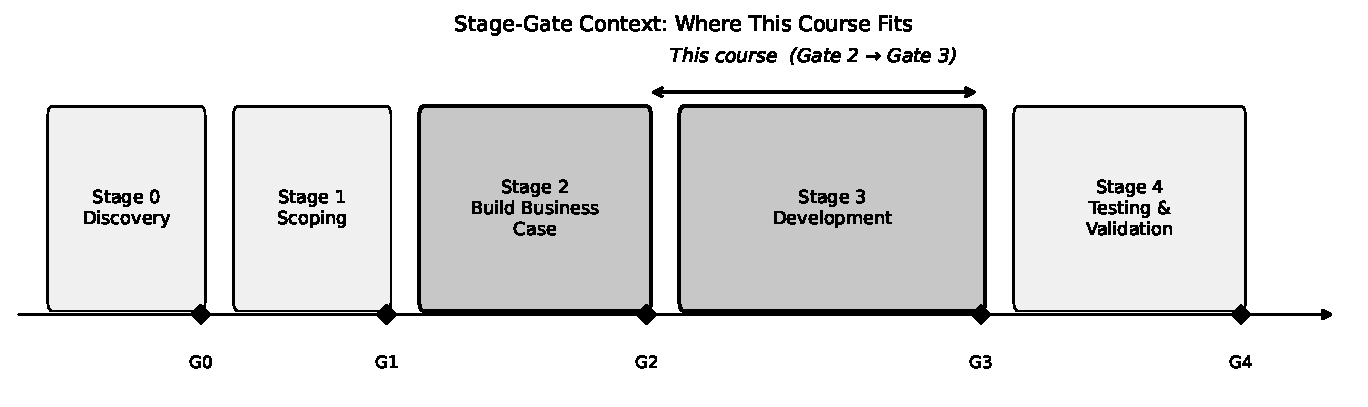
\includegraphics[width=0.92\textwidth]{images/fig_01_stagegate_course}
\caption{The course spans Stage~2 (Build Business Case) and Stage~3 (Development),
         exiting at Gate~3 with a validated prototype.}
\label{fig:cp-stagegate}
\end{figure}

\section*{12-Week Timeline}
\addcontentsline{toc}{section}{12-Week Timeline}

\begin{figure}[h]
\centering
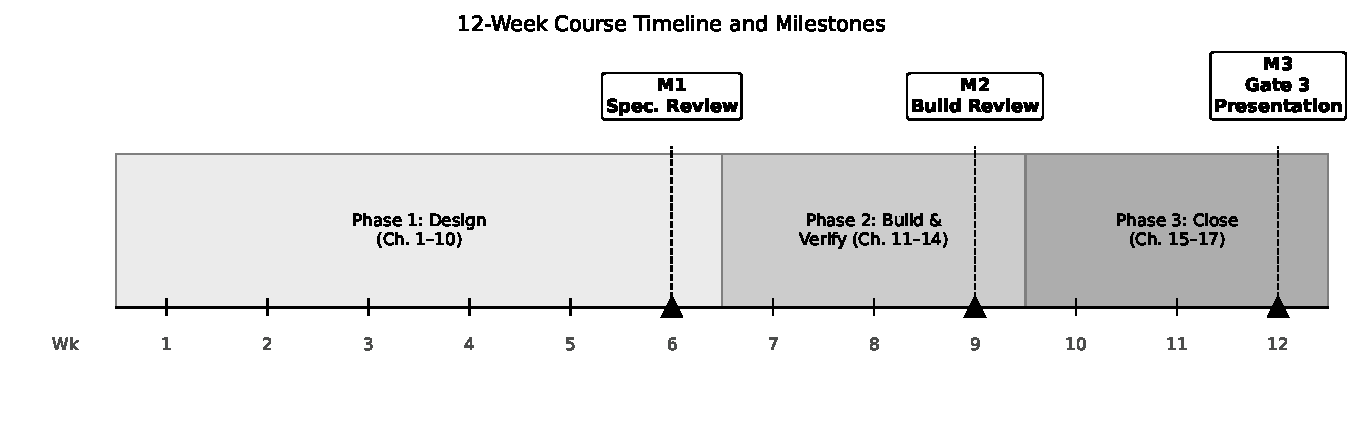
\includegraphics[width=0.92\textwidth]{images/fig_02_milestone_timeline}
\caption{Three course phases and milestone dates. Each phase closes with a graded
         submission.}
\label{fig:cp-timeline}
\end{figure}

\newpage

\section*{Weekly Schedule}
\addcontentsline{toc}{section}{Weekly Schedule}

The table below lists lecture topics, associated textbook chapters, lab activities,
and the Portfolio Entry due at the end of each week.
Lab sessions (2~h) are used to work on the current Portfolio Entry under instructor
supervision.

\begin{longtable}{@{}
    >{\bfseries\centering\arraybackslash}p{0.8cm}   % Week
    L{2.8cm}                                          % Topic
    L{1.4cm}                                          % Chapter(s)
    L{3.6cm}                                          % Lab / Activity
    L{3.8cm}                                          % Deliverable
    @{}}
\toprule
\textbf{Week} & \textbf{Topic} & \textbf{Ch.} & \textbf{Lab Activity} & \textbf{Deliverable} \\
\midrule
\endfirsthead
\multicolumn{5}{l}{\small\itshape (continued from previous page)} \\
\toprule
\textbf{Week} & \textbf{Topic} & \textbf{Ch.} & \textbf{Lab Activity} & \textbf{Deliverable} \\
\midrule
\endhead
\bottomrule
\endfoot
\bottomrule
\endlastfoot

1 &
Course introduction; product vs.\ prototype; revenue models; gross margin &
1 &
Project kick-off: choose design project; compute $m$ and GM\% for three revenue scenarios &
Portfolio Entry~1: Project Context Brief \\[4pt]

2 &
Stage-Gate model; Kano model; voice-of-customer mapping &
2 &
Map five customer needs to Kano categories; identify must-be and performance attributes &
Portfolio Entry~2: Stage-Gate + Kano Analysis \\[4pt]

3 &
Seven-stage prototyping workflow; fidelity ladder; effort model $E(f) = E_0 \cdot k^f$ &
3 &
Select fidelity level for your project PoC; compute effort ratio $E(5)/E(2)$ &
Portfolio Entry~3: Workflow Plan \\[4pt]

4 &
Writing engineering specifications; MoSCoW; tolerance vs.\ requirement &
4 &
Draft five MoSCoW specifications for your project; set measurable pass/fail criteria &
Portfolio Entry~4: Specification Table \\[4pt]

5 &
System architecture; block diagrams; interface definition; specify-and-trust vs.\ prototype &
5 &
Draw block diagram; classify each subsystem using the three-question decision flow &
Portfolio Entry~5: System Architecture \\[4pt]

6 &
Component selection; datasheet reading; supplier comparison; risk ranking &
6 &
Build a three-candidate comparison table for one key component; select and justify &
Portfolio Entry~6: Component Selection \\[4pt]

\midrule
\multicolumn{5}{c}{\textbf{Milestone 1 --- Specification Review (end of Week~6)}} \\
\multicolumn{5}{c}{\small Assemble Portfolio Entries 1--6; submit as one PDF.
                          All design decisions locked from this point.} \\
\midrule

7 &
Design for manufacturing; DFM, DFA, DFT principles; cost-of-change curve &
7 &
Apply DFM checklist to your PCB layout; identify one DFM improvement &
Portfolio Entry~7: DFX Review \\[4pt]

8 &
AI integration; edge inference; model selection; latency and accuracy trade-offs &
8 &
Run a pre-trained model on target hardware; measure inference latency &
Portfolio Entry~8: AI Integration Notes \\[4pt]

9 &
IoT and robotics integration; communication protocols; power budgeting; safety &
9 &
Build power budget table for your project; identify single-point failure modes &
Portfolio Entry~9: IoT/Robotics Integration \\[4pt]

\midrule
\multicolumn{5}{c}{\textbf{Milestone 2 --- Build Review (end of Week~9)}} \\
\multicolumn{5}{c}{\small Prototype operational; add Portfolio Entries 7--9 to package.
                          Instructor sign-off required.} \\
\midrule

10 &
Project planning; PERT; Gantt charts; critical path &
10 &
Build a five-task PERT network; compute $t_e$ and $\sigma^2$ for each task &
Portfolio Entry~10: Project Schedule \\[4pt]

11 &
BOM and procurement; as-built BOM; supplier lead times; RFQ process &
11 &
Update your BOM with actual component costs; flag lead-time risks &
Portfolio Entry~11: As-Built BOM \\[4pt]

12 &
Engineering economics; break-even; fixed vs.\ variable cost; GM\% sensitivity &
12 &
Compute $N^*$ and GM\% for your project at three production volumes &
Portfolio Entry~12: Cost Analysis \\[4pt]

13 &
Version control and design history file; DHF structure; change-control log &
13 &
Set up a Git repository; write one ECO entry for a design change &
Portfolio Entry~13: Version Control Setup \\[4pt]

14 &
Validation testing; statistical process control; fault tree analysis &
14 &
Run 10 measurements of a key spec; compute $\bar{x}$, $s$, $z$, $C_p$ &
Portfolio Entry~14: Validation Report \\[4pt]

15 &
Intellectual property; patents; trade secrets; NDAs; prior-art search &
15 &
Complete IP checklist for your project; identify one protectable element &
Portfolio Entry~15: IP Checklist \\[4pt]

16 &
Documentation assembly; traceability matrix; requirements coverage; DHF review &
16 &
Complete the 14-section portfolio package; run coverage audit &
Portfolio Entry~16: Complete Documentation Package \\[4pt]

17 &
Cost bridge to production; unit-cost hyperbola; revenue break-even $N_\mathrm{be}$;
Gate~3 readiness statement &
17 &
Compute $C_\mathrm{unit}$ at $N = 1$, 50, 500; write Gate~3 readiness statement &
Portfolio Entry~17: Cost Projection + Gate~3 Statement \\[4pt]

\midrule
\multicolumn{5}{c}{\textbf{Milestone 3 --- Gate~3 Presentation (end of Week~12 exam period)}} \\
\multicolumn{5}{c}{\small 10--15 min live presentation + complete documentation package.
                          This is the Gate~3 exit submission.} \\

\end{longtable}

\section*{Evaluation Summary}
\addcontentsline{toc}{section}{Evaluation Summary}

\begin{tabular}{@{}lll@{}}
\toprule
\textbf{Assessment} & \textbf{Weight} & \textbf{Due} \\
\midrule
Milestone~1 --- Specification Review       & 20\% & End of Week~6 \\
Milestone~2 --- Build Review               & 20\% & End of Week~9 \\
Weekly Portfolio Entries (10--16, 17)      & 25\% & Each week (lab submission) \\
Milestone~3 --- Gate~3 Presentation       & 35\% & Exam period \\
\midrule
\textbf{Total}                             & \textbf{100\%} & \\
\bottomrule
\end{tabular}

\bigskip

\noindent\textbf{Portfolio Entry policy.}\quad
Each Portfolio Entry is submitted at the end of its lab session.
Entries submitted late without prior arrangement are capped at 50\%.
Entries are cumulative: later submissions may revise earlier ones in response to
instructor feedback, provided the revised section is clearly marked
\texttt{[Rev.\ N, date]}.

\section*{Required Materials}
\addcontentsline{toc}{section}{Required Materials}

\begin{itemize}
\item \textit{Project Planning \& Prototyping} (this textbook), J. F. N. Salik, 2026.
      Available on Lea / Moodle as PDF.
\item A prototyping kit issued at the start of term (contents listed in Ch.~6 BOM).
\item Laptop capable of running Python~3 and KiCad~8.
\item GitHub account (free); Git client installed locally.
\end{itemize}

\section*{SPLI Note}
\addcontentsline{toc}{section}{SPLI Note}

This course is structured to support \emph{Self-Paced Learning Integration} (SPLI).
Students who complete a chapter's Portfolio Entry to a passing standard before the
scheduled week may proceed to the next chapter independently.
Milestone dates are fixed for all students regardless of pace.
Students working ahead are encouraged to iterate on earlier Portfolio Entries
using subsequent chapters' methods.

\end{document}
